    \begin{figure} 
      \centering
      \subfloat[][$e=1$.]{\noindent
        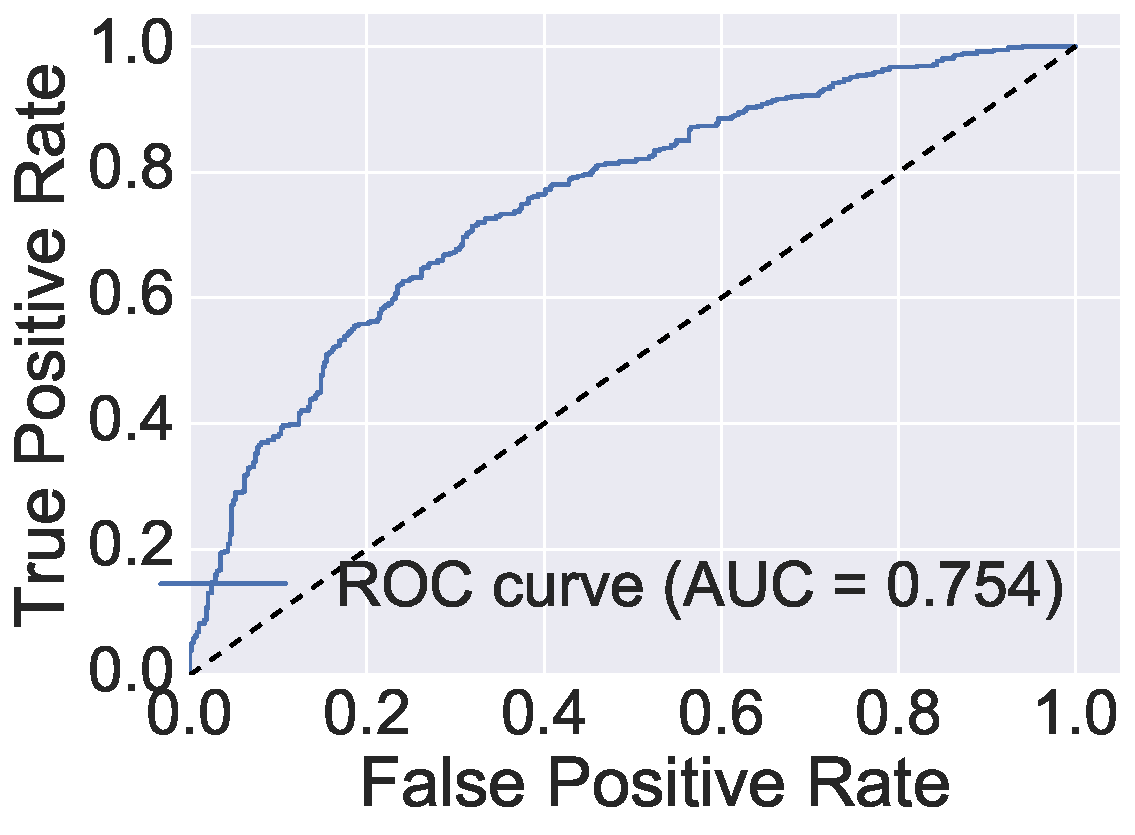
\includegraphics[width=.4\textwidth]{/Users/ijoseph/Documents/Work/Graduate-Thesis/TeX/figures/ch4/n_1000/mfaa__roc__w_2_psi_2.pdf}}% 
      \qquad \\
      \subfloat[][$e=1.25$.]{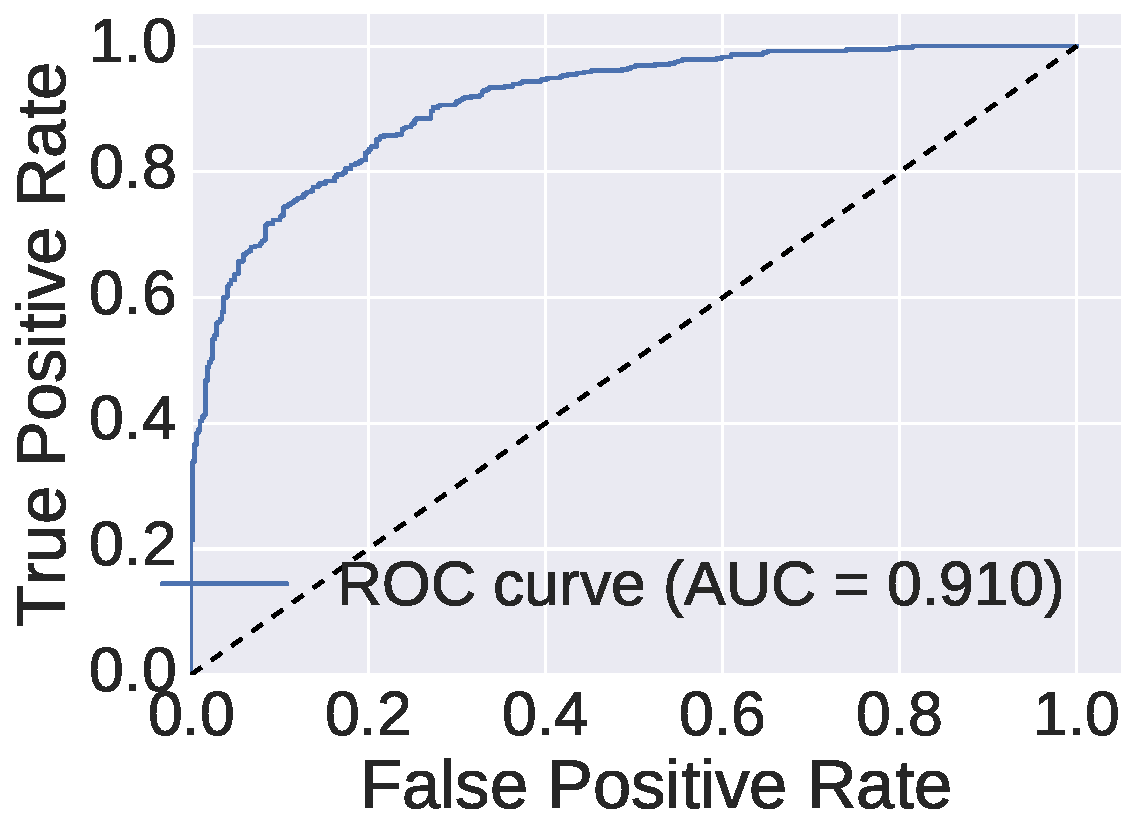
\includegraphics[width=.4\textwidth]{{/Users/ijoseph/Documents/Work/Graduate-Thesis/TeX/figures/ch4/n_1000/mfaa__roc__w_3_psi_2}.pdf}}
      \qquad \\
      \subfloat[][$e=10$.]{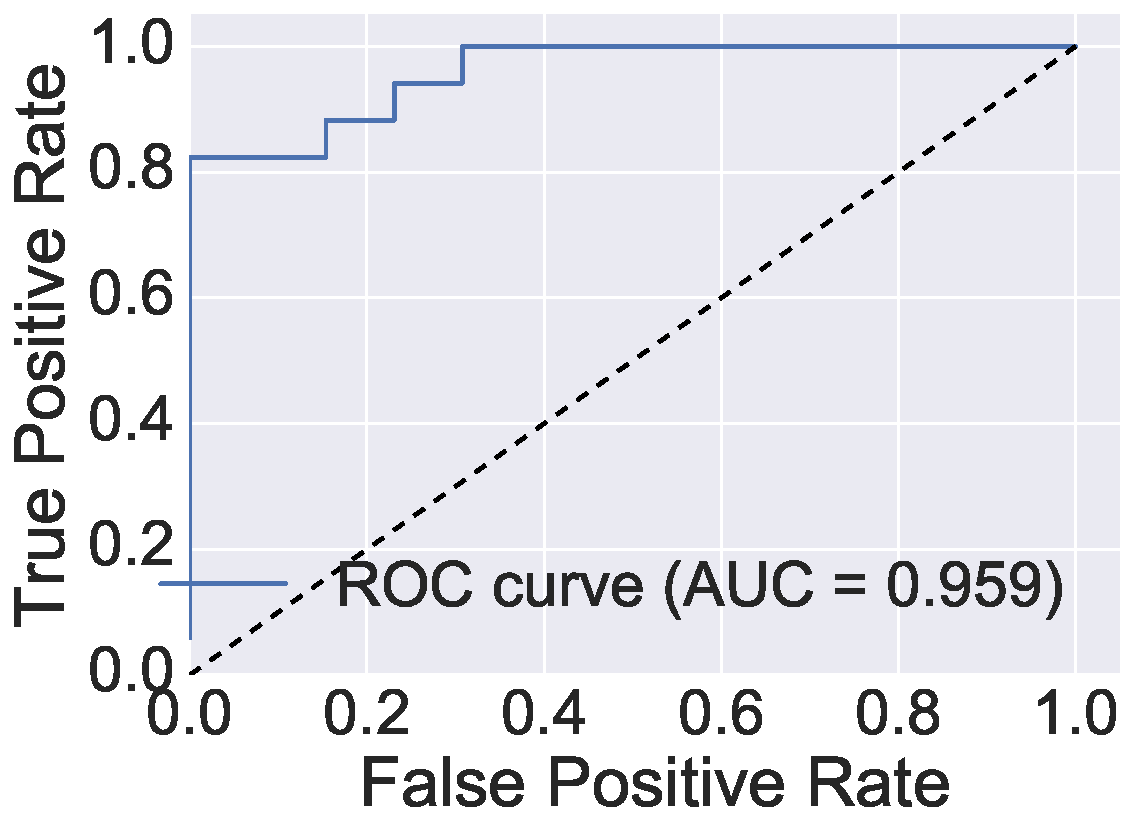
\includegraphics[width=.4\textwidth]{{/Users/ijoseph/Documents/Work/Graduate-Thesis/TeX/figures/ch4/n_1000/mfaa__roc__w_20_psi_2}.pdf}}
      \caption{HFAM ROC curves from HFAM-simulated $N=1000, p=10$.} \label{fourthreeone}
    \end{figure}

    \begin{figure} 
      \centering
      \subfloat[][$e=1$.]{\noindent
        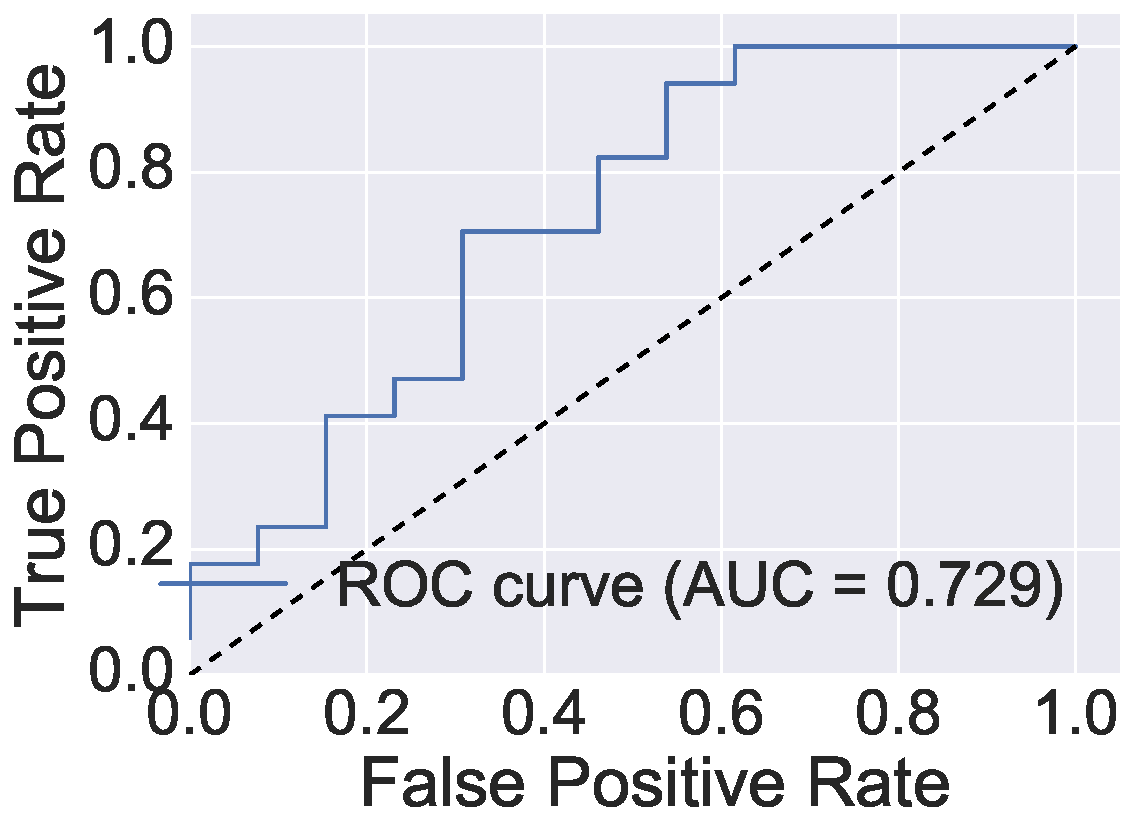
\includegraphics[width=.4\textwidth]{/Users/ijoseph/Documents/Work/Graduate-Thesis/TeX/figures/ch4/n_1000/log_reg__roc__w_2_psi_2.pdf}}% 
      \qquad \\
      \subfloat[][$e=1.25$.]{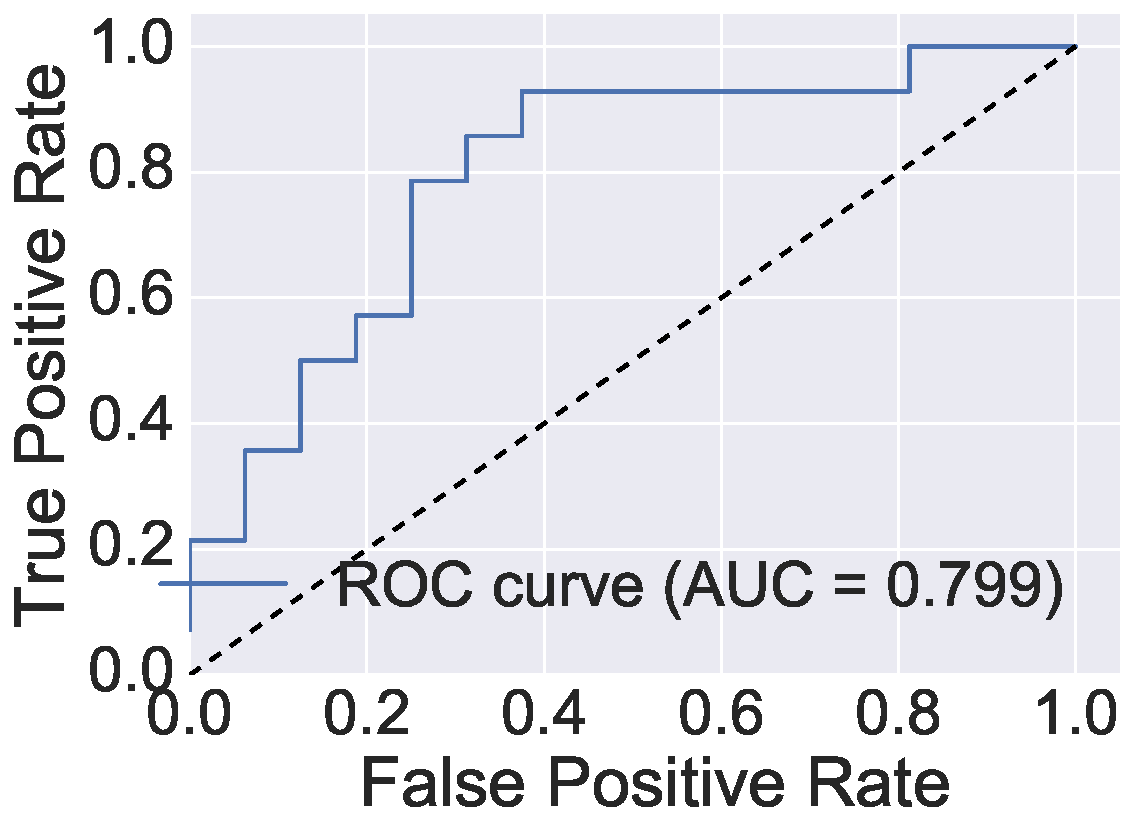
\includegraphics[width=.4\textwidth]{{/Users/ijoseph/Documents/Work/Graduate-Thesis/TeX/figures/ch4/n_1000/log_reg__roc__w_3_psi_2}.pdf}}
      \qquad \\
      \subfloat[][$e=10$.]{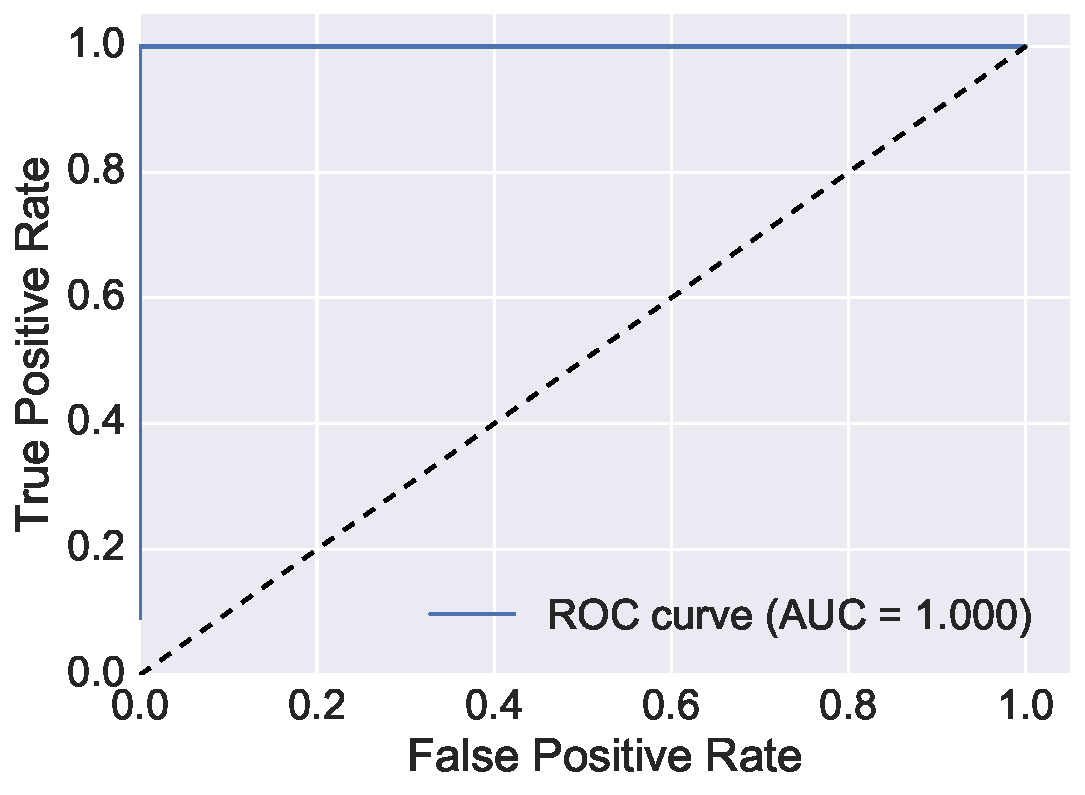
\includegraphics[width=.4\textwidth]{{/Users/ijoseph/Documents/Work/Graduate-Thesis/TeX/figures/ch4/n_1000/log_reg__roc__w_20_psi_2}.pdf}}
      \caption{Logistic regression ROC curves from HFAM-simulated
        $N=1000, p=10$.} \label{fourthreetwo}
    \end{figure}    


    \begin{figure} 
      \centering
      \subfloat[][$e=1$.]{\noindent
        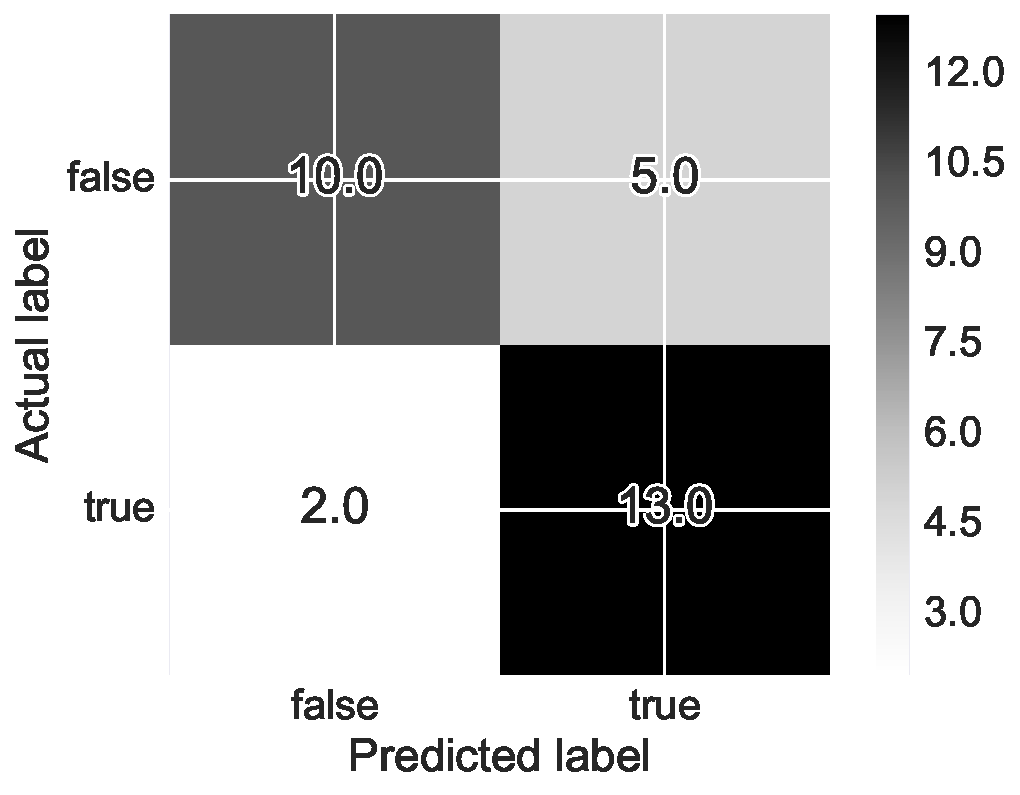
\includegraphics[width=.4\textwidth]{/Users/ijoseph/Documents/Work/Graduate-Thesis/TeX/figures/ch4/n_1000/mfaa__confusion__w_2_psi_2.pdf}}% 
      \qquad \\
      \subfloat[][$e=1.25$.]{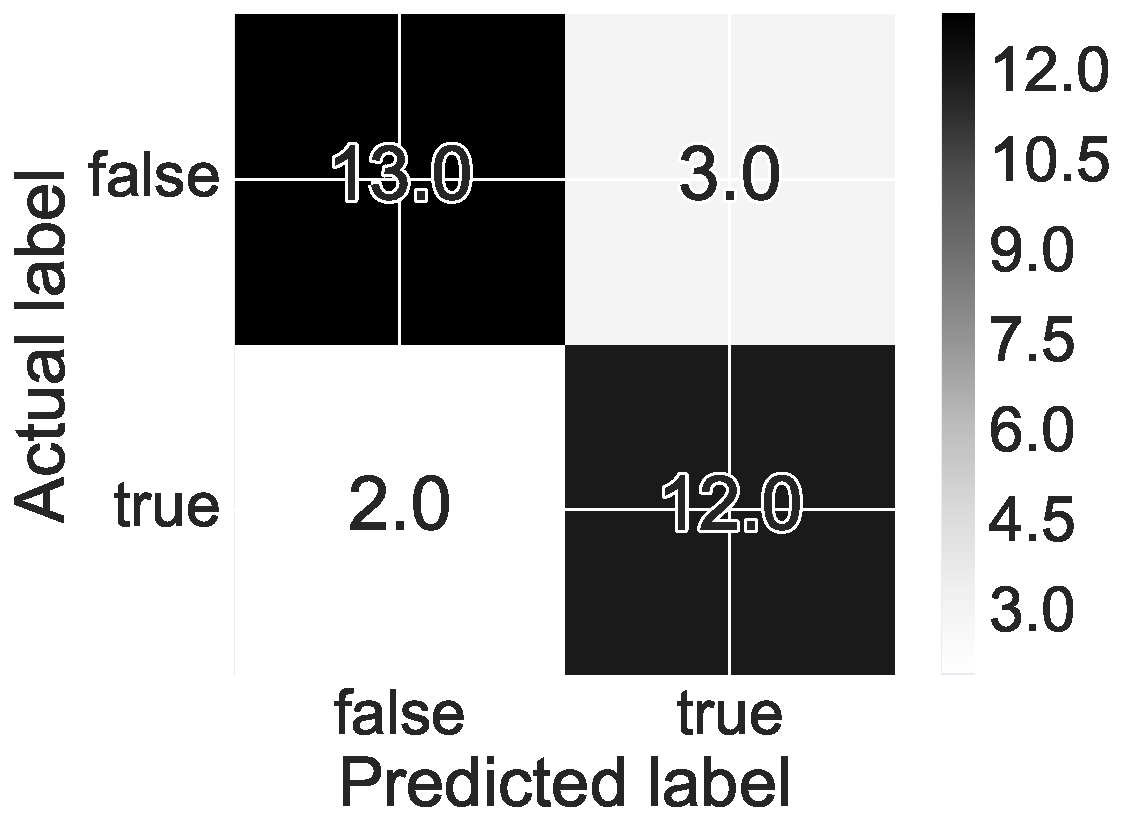
\includegraphics[width=.4\textwidth]{{/Users/ijoseph/Documents/Work/Graduate-Thesis/TeX/figures/ch4/n_1000/mfaa__confusion__w_3_psi_2}.pdf}}
      \qquad \\
      \subfloat[][$e=10$.]{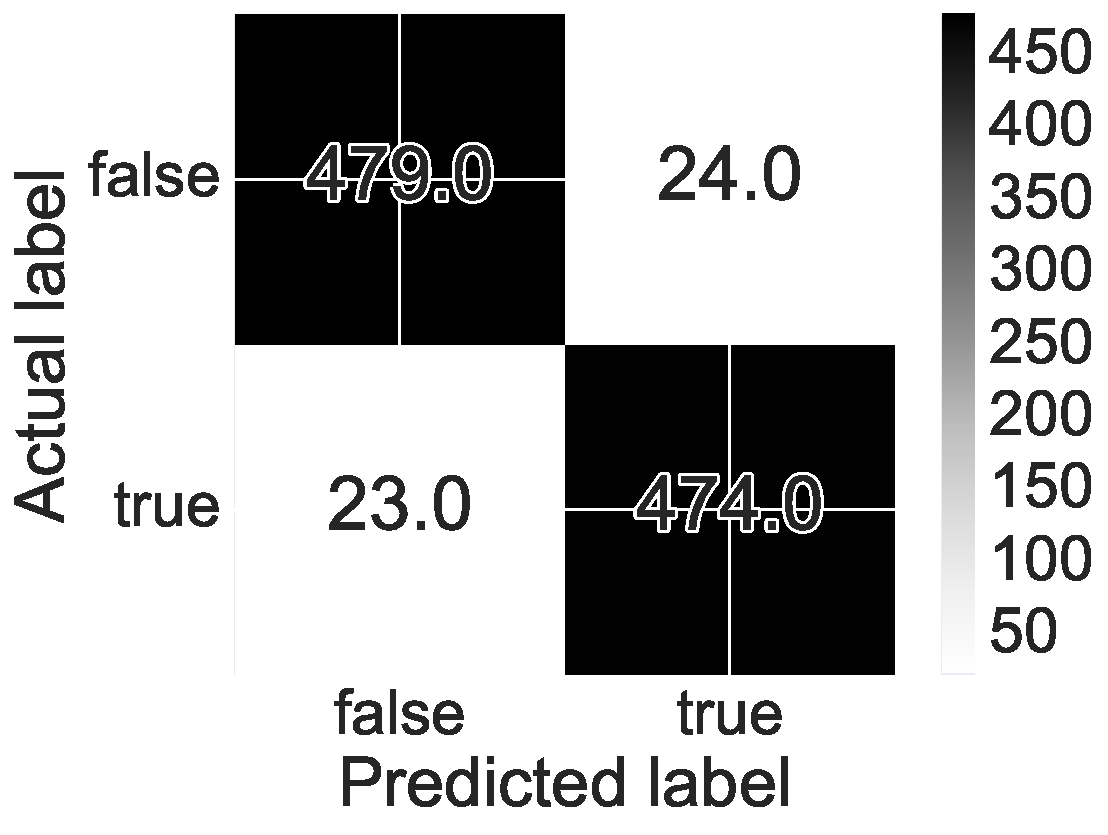
\includegraphics[width=.4\textwidth]{{/Users/ijoseph/Documents/Work/Graduate-Thesis/TeX/figures/ch4/n_1000/mfaa__confusion__w_20_psi_2}.pdf}}
      \caption{HFAM confusion matrices from HFAM-simulated $N=1000,
        p=10$.} \label{fourthreethree}
    \end{figure}


    \begin{figure} 
      \centering
      \subfloat[][$e=1$.]{\noindent
        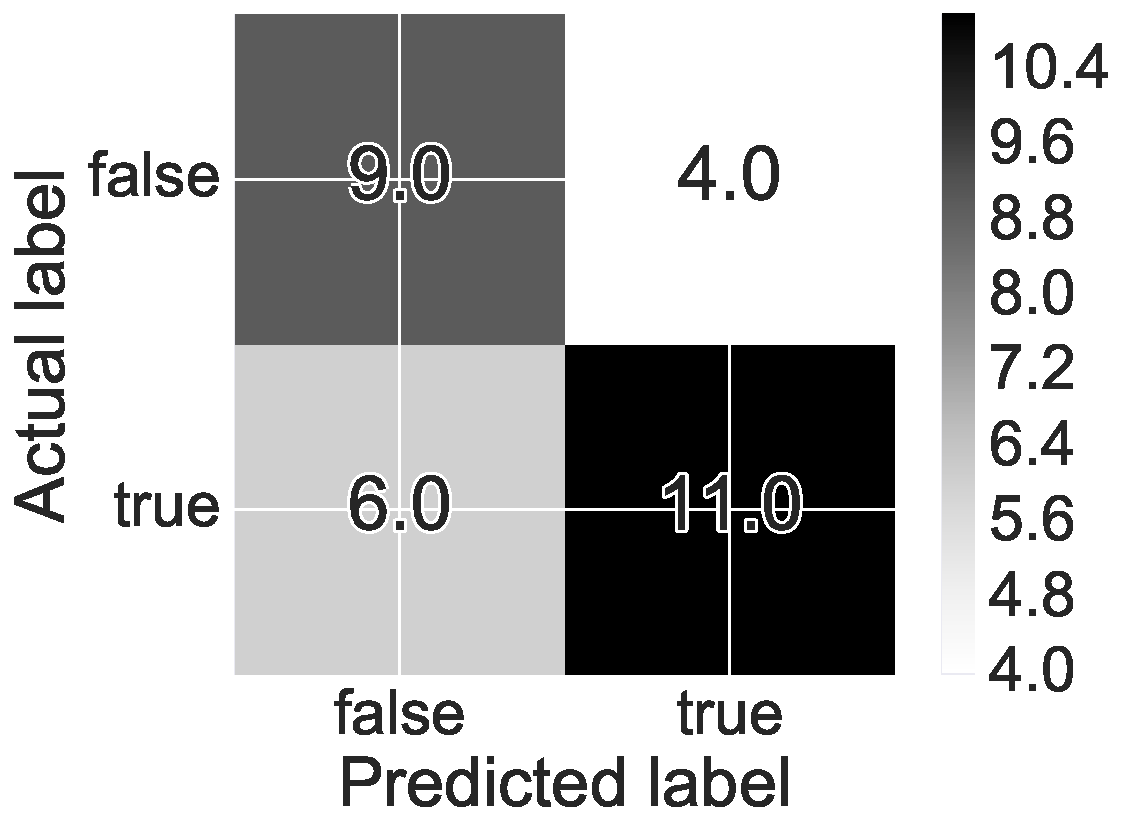
\includegraphics[width=.4\textwidth]{/Users/ijoseph/Documents/Work/Graduate-Thesis/TeX/figures/ch4/n_1000/log_reg__confusion__w_2_psi_2.pdf}}% 
      \qquad \\
      \subfloat[][$e=1.25$.]{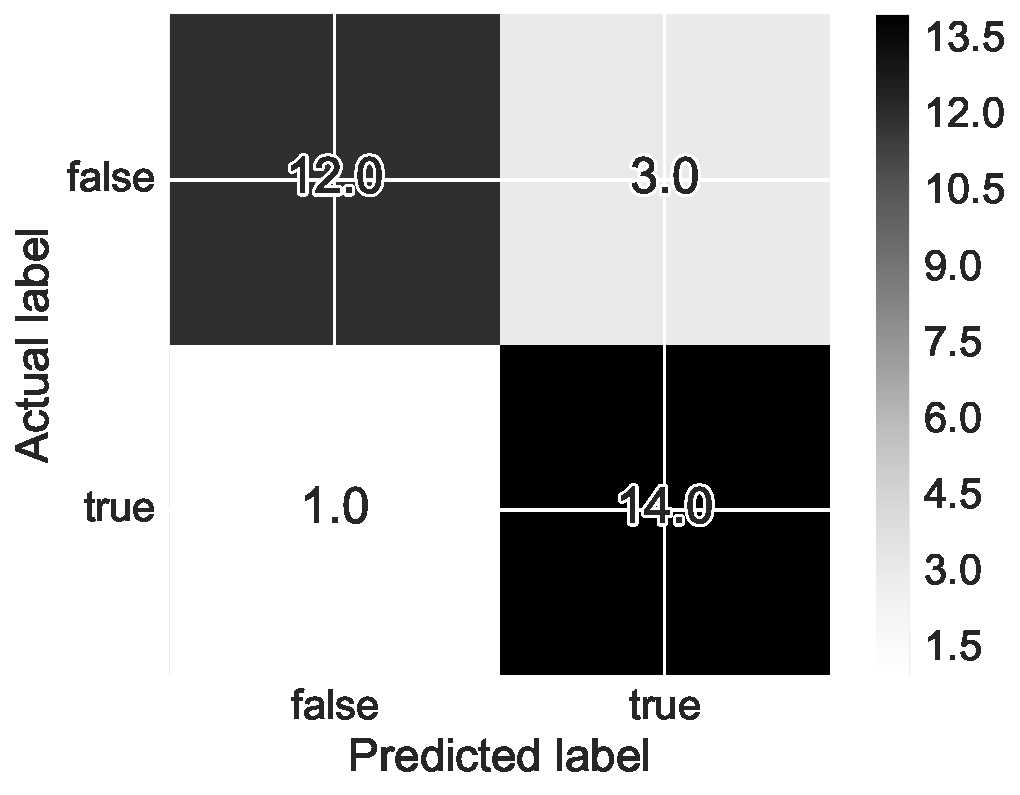
\includegraphics[width=.4\textwidth]{{/Users/ijoseph/Documents/Work/Graduate-Thesis/TeX/figures/ch4/n_1000/log_reg__confusion__w_3_psi_2}.pdf}}
      \qquad \\
      \subfloat[][$e=10$.]{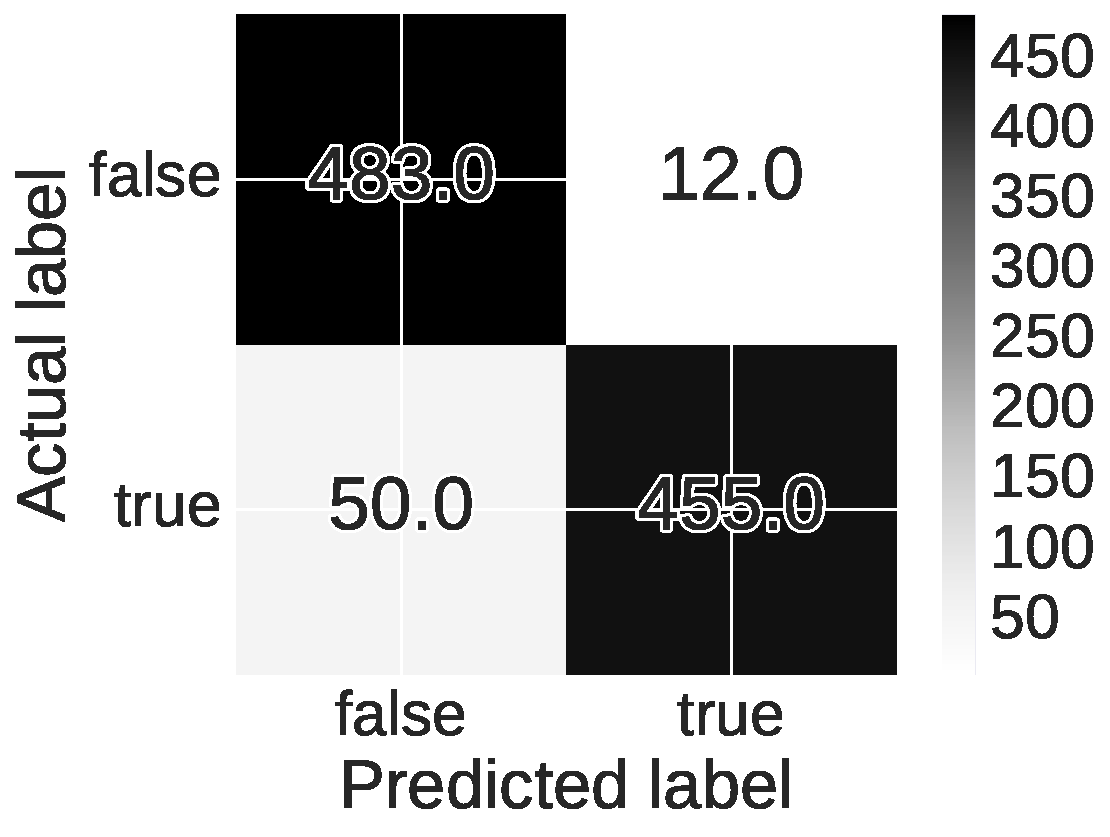
\includegraphics[width=.4\textwidth]{{/Users/ijoseph/Documents/Work/Graduate-Thesis/TeX/figures/ch4/n_1000/log_reg__confusion__w_20_psi_2}.pdf}}
      \caption{Logistic regression confusion matrices from
        HFAM-simulated $N=1000, p=10$.} \label{fourthreefour}
    \end{figure}




    
    


    





